%\documentclass[handout]{beamer}
\documentclass{beamer}

% Customize slide appearance
\mode<presentation>
{
  \usetheme{default}
%  \setbeamercovered{transparent}
}

\usepackage[english]{babel}
\usepackage{times}
\usepackage{threeparttable}
\usepackage{tabularx}
\usepackage{booktabs}
\usepackage{pgfpages}
\usepackage{latexsym,amsmath,amssymb,textcomp,eurosym,dcolumn,booktabs}
\usepackage{color}
\usepackage{colortbl}
\usepackage{graphicx}
\usepackage{amsthm}

\definecolor{darkblue}{rgb}{0.1,0,0.55} \definecolor{darkgreen}{rgb}{0,0.7,0}
\definecolor{important}{rgb}{0.9,0.1,0.1} %
\definecolor{hidden}{rgb}{0.8,0.8,0.8}
\definecolor{darkgreen}{rgb}{0,0.7,0}

\usenavigationsymbolstemplate{}
\setbeamertemplate{footline}
    {\begin{beamercolorbox}[sep=1ex]{author in head/foot}
      \hfill\llap{\insertframenumber}%
      \end{beamercolorbox}%
      }


%\pgfpagesuselayout{4 on 1}



\AtBeginSection[]
{
  \begin{frame}
  \frametitle{Outline}
  \large{\tableofcontents[currentsection,hideothersubsections]}
  \end{frame}
}


%\usepackage{amstext}

\begin{document}

\begin{frame}

\bigskip

\center{{\Large \textcolor{darkblue}{Seeing is Believing: \\ Identity, Inequality, and the Impact of Television on the Hispanic Achievement Gap}} \medskip}

\bigskip


\center{\textbf{Andrew Kao} \\ \textit{Harvard}}

\bigskip \bigskip

\center{February 2022}

\end{frame}


%%%%% MOTIVATION %%%%%%
\begin{frame}
\frametitle{Motivation}


\begin{itemize}

\item Hispanics in the US face large obstacles. Compared to white people, they are:
\begin{itemize}
\item \textbf{60\%} less likely to complete college,
\item \textbf{68\%} less likely to found a business,
\item and have \textbf{5x} less household wealth (\$38k vs. \$148k)
\end{itemize}
\pause
\item Americans spend more time watching TV than any other activity but sleep
\begin{itemize} 
\item \textbf{50\%} of Hispanics watch satellite or broadcast Spanish Language TV (SLTV) 
\end{itemize}
\pause 
\item Large literature on how TV affects behavior {\footnotesize(\textbf{Gentzkow \& Shapiro 2008}; DellaVigna \& al. 2007;  Ferrara \&\ al., 2012)}
\item Prior efforts to study Hispanic interaction with media focused on politics {\footnotesize(Waldfogel \& al. 2009; Trujillo \& al. 2012)}
\end{itemize}

\end{frame}


%%%%% PROJECT OVERVIEW %%%%%%
\begin{frame}
\frametitle{This project:}

Show that SLTV reduces the Hispanic achievement gap in public schools:
\begin{itemize}
\item Identification: difference-in-discontinuities design
\item Gap vs. whites and Asians in SAT/ACTs taken, calculus courses taken, AP exams passed, etc. \textbf{shrinks} with SLTV
\item However, the gap vs. whites and Asians \textbf{rises} when looking at English proficiency
\end{itemize}

How to reconcile this?
\pause 
Propose an \textbf{identity} mechanism. Three strands of evidence:

\begin{enumerate}
\item More bullying on the basis of ethnicity (but not gender)

\item Hispanics in places where SLTV focuses more Hispanic identity perform better (but not if SLTV focuses more on education)

\item Hispanics with SLTV visit Hispanic branded establishments more (but not Brazilian branded ones)

\end{enumerate}

\end{frame}

%%% DATA %%%

\begin{frame}
\frametitle{Data - General}

\begin{itemize}
\item Instrument:
\begin{itemize}
\item Identify 100 Spanish Language TV stations across the US from TMS
\item Station contours and other station data from the FCC (use data from 2015 for consistency with outcomes)
\end{itemize}
\item Geocoding:
\begin{itemize}
\item ArcGIS: 99.9\%+ successfully geocoded
\end{itemize}
\item Demographic information at county/census block group level from ACS
\end{itemize}

\end{frame}



%%% COVERAGE MAP %%%
\begin{frame}
\frametitle{Coverage Map for TV Station WUVC-DT}
\centering
        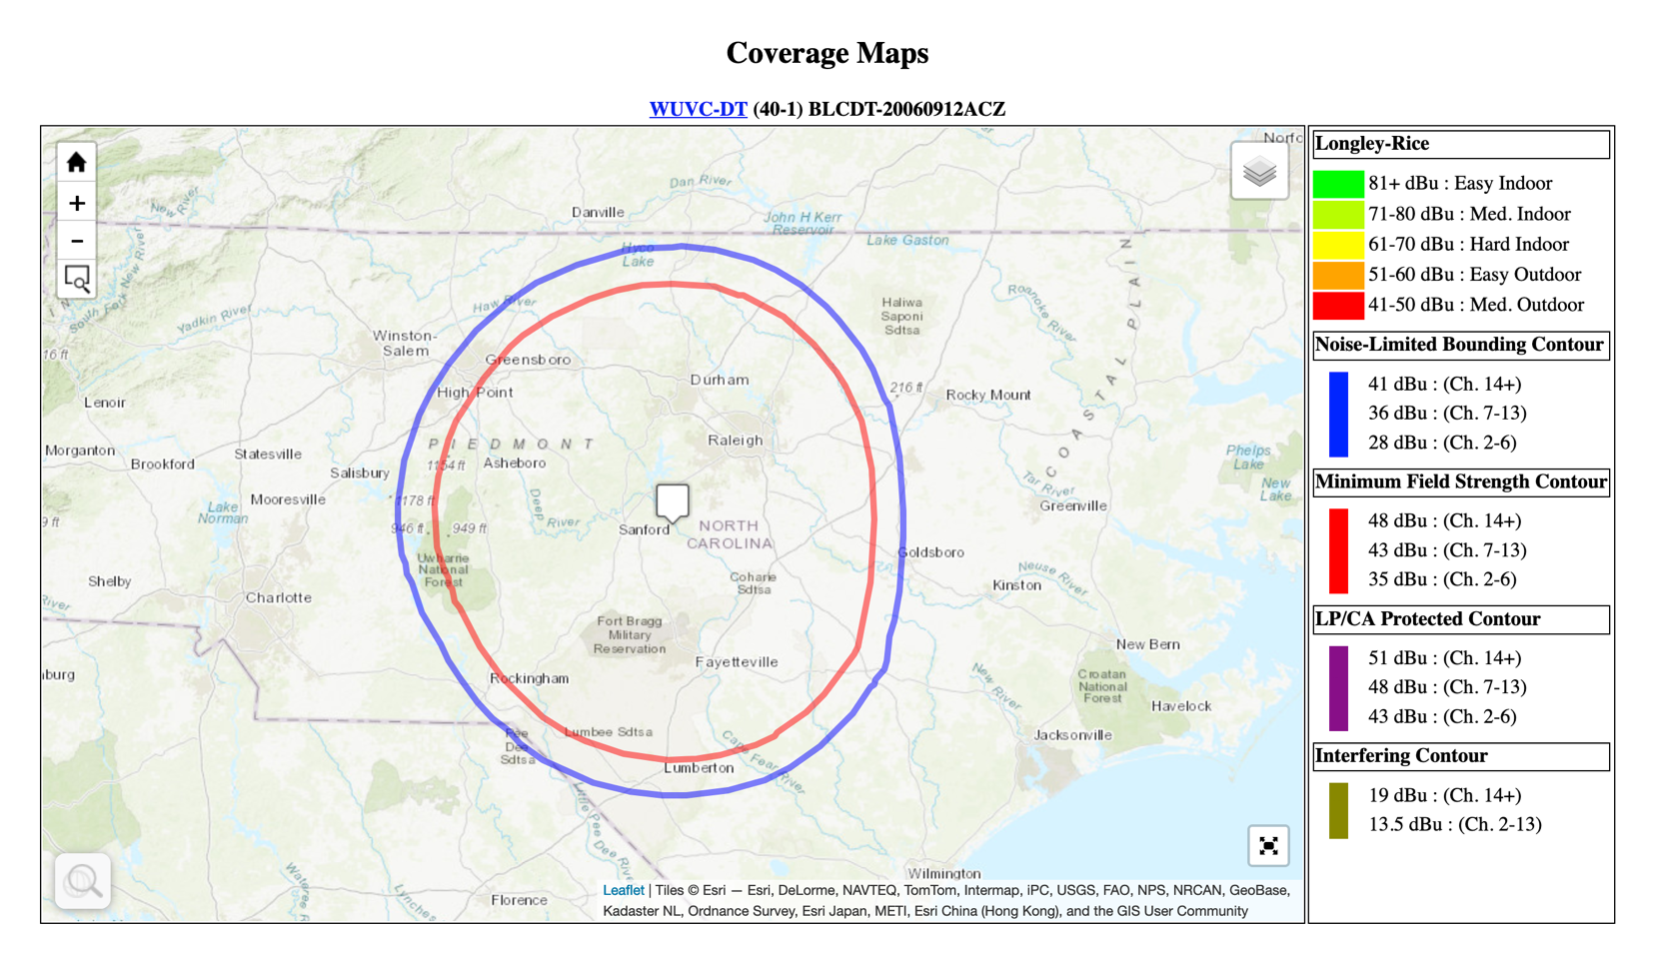
\includegraphics[width=1\textwidth]{../../analysis/Output/img/ContourExample.png}\\
\end{frame}

%%% EMPIRICAL STRATEGY %%%
\begin{frame}
\frametitle{Empirical Strategy}
\begin{itemize}
\item Follow Velez \& Newman (2019) and construct spatial RD arising from FCC TV signal regulation (OET Bulletin 69)
\item TV stations protected from interference within certain coverage contour areas. Keep observations within 100 KM of boundary
\begin{itemize}
\item Mechanical formula based on geographic/technical factors (not political/economic)
\item Fairly large contour areas, boundaries typically cut through small towns/suburbs
\item Most stations constructed prior to 1997 when this regulation was implemented
\end{itemize}
\item Spanish Language TV: Isolate effect on Hispanic communities

\pause
\item Compare against outcomes among Asians
\begin{itemize}
\item Less likely to identify as Hispanic (or watch SLTV)
\item Combine RD with Asian `control' for difference in discontinuities
\end{itemize}

\end{itemize}

\end{frame}


%%% COUNTRY MAP %%%
\begin{frame}
\frametitle{SLTV coverage and public schools}
\centering
        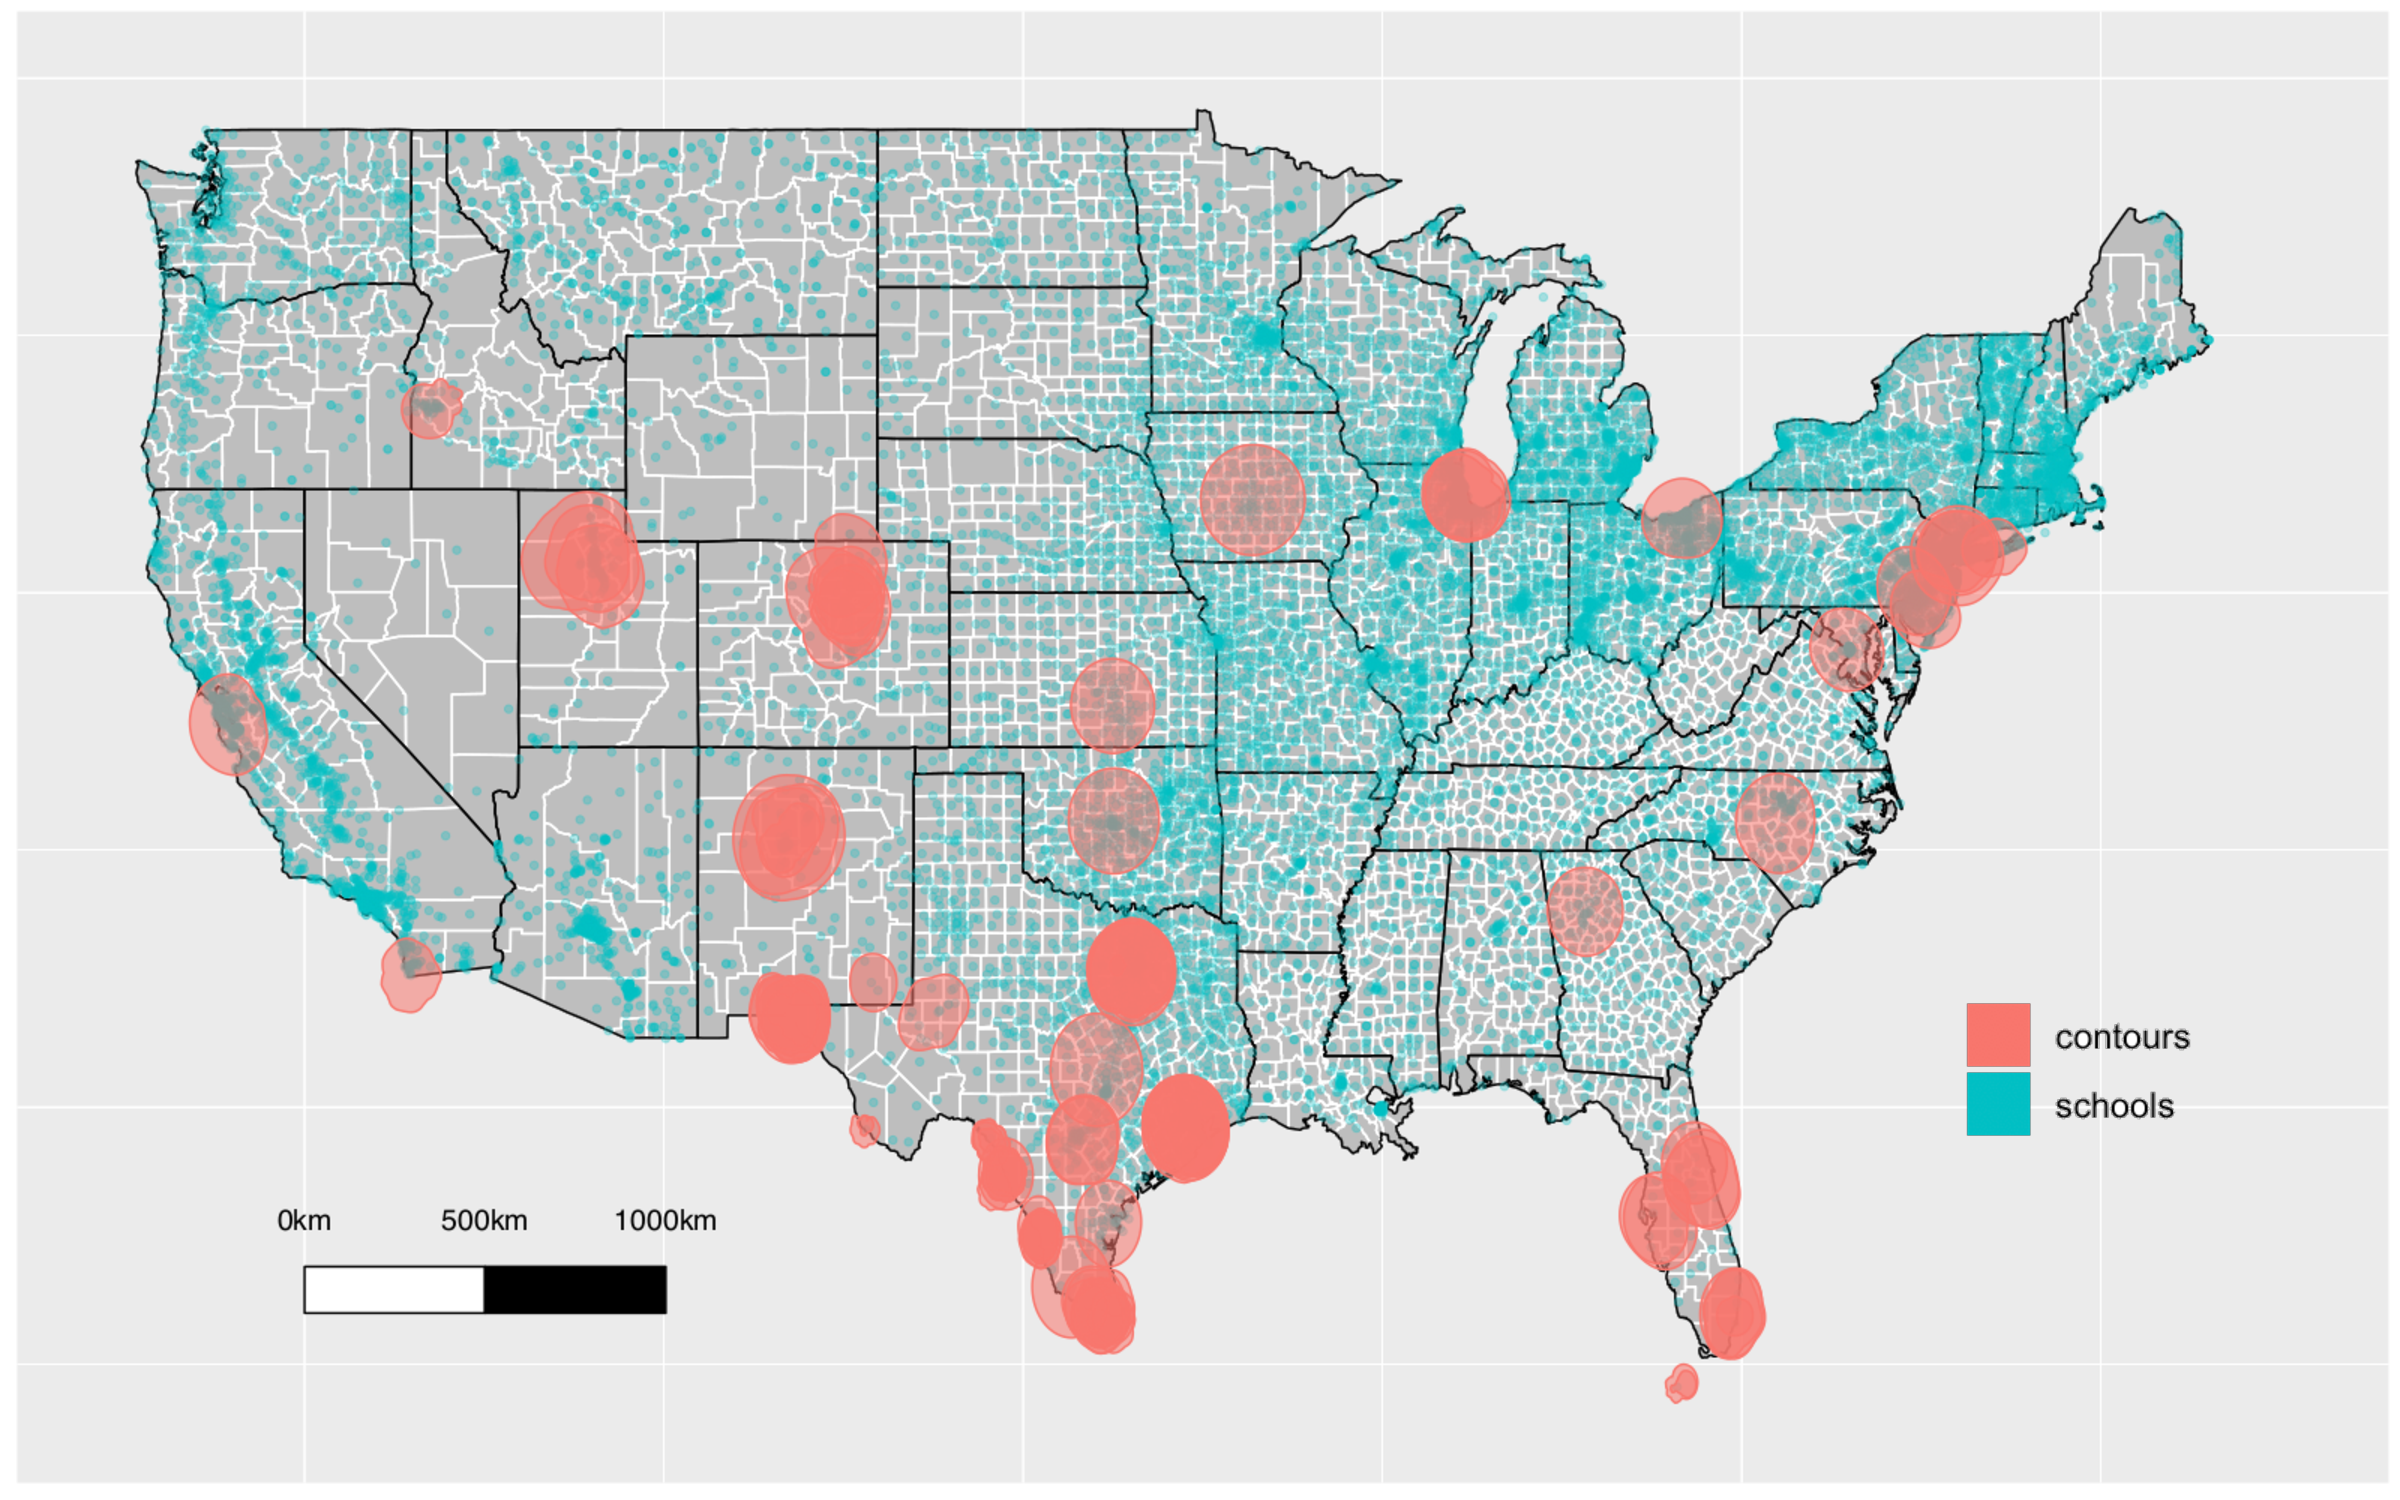
\includegraphics[width=1\textwidth]{../../analysis/Output/img/Schools_pretty2.pdf}\\
\end{frame}

%%% SPECIFICATIONS %%%
\begin{frame}
\frametitle{Empirical Specification}

\[ y_{i,j} =  \beta \mathbb{I}[InsideContour_{i,j}] \times \mathbb{I}[Hispanic_{i,j}] + \gamma_k + \delta  X_i + \epsilon_{i,j} \]

\vspace{5pt}

where $y_{i,j}$ is an outcome for observation $i$ (which may be an individual, school, or establishment) under demographic category $j \in \{$Hispanic, not Hispanic$\}$, $\gamma_k$ is fixed effect for school district $k$, and $X$ is a vector of controls for the observation. 


\end{frame}








%%%% FIRST STAGE %%%%%

\begin{frame}
\frametitle{Evidence of first stage}

\begin{itemize}

\item Data from American Time Use Survey over last 15 years:
\begin{itemize}
\item 210,000 person-year observations
\item Average person watches 170 minutes of TV per day
\end{itemize}

\vspace{10pt}
\item Two limitations:
\begin{itemize}
\item County-level data is noisy for RD approach
\item Only overall TV viewership data, not SLTV
\end{itemize}

\end{itemize}

\end{frame}




\begin{frame}
\frametitle{TV Viewership within the SLTV Boundary} \label{atus_time}

\begin{center}
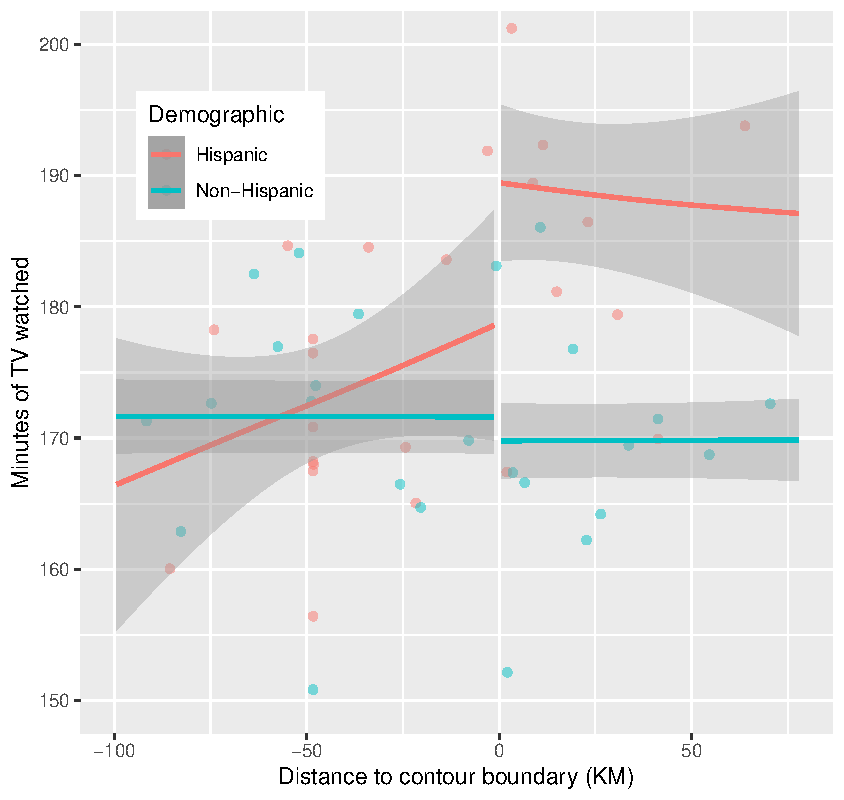
\includegraphics[width=.75\textwidth]{../../analysis/Output/graphs/atus2.pdf}\\
\end{center}
\vspace{-5pt}
\footnotesize Negative distances are outside coverage contour (no SLTV). \hyperlink{atus_breakdown}{\beamergotobutton{Time breakdown}}

%\begin{center}
%\scalebox{.8}{
%	\begin{threeparttable}
%			\begin{tabular}{lcccccccccc}
%				\hline\hline\addlinespace
%				Panel A: Minutes of TV watched &  (1) & (2) & (3) & (4) \\
%                                \hline\addlinespace
% TV Dummy $\times$ Hispanic  & 13.610$^{***}$ & 14.638$^{***}$ & 8.777$^{**}$ & 7.911$^{**}$ \\ 
%  & (3.825) & (3.831) & (3.834) & (3.829) \\ 
% TV Dummy & $-$1.170 & $-$1.392 & 4.096$^{**}$ & 5.030$^{**}$ \\ 
%  & (1.944) & (1.945) & (1.960) & (1.958) \\ 
%Observations & 91,315 & 91,315 & 91,315 & 91,315 \\              
%\hline\hline\addlinespace
%County \% Hispanic & No & Yes & Yes & Yes \\
%Log(Income) & No & No & Yes & Yes \\
%Person is Migrant & No & No & No & Yes \\
%				\addlinespace\hline\hline
%			\end{tabular}
%			\begin{tablenotes}[flushleft]
%				\item \textit{Notes:} 
%			\end{tablenotes}
%		\end{threeparttable}
%        }
%\end{center}
 

\end{frame}


%%%%%% SCHOOLS %%%%%%
\begin{frame}

\huge {\color{darkblue} Effect of SLTV on the Hispanic achievement gap}

\end{frame}



\begin{frame}
\frametitle{Data: public schools}
\begin{itemize}
\item Data from Department of Education's Civil Rights Data Collection in 2015:
\begin{itemize}
\item 48,000 public schools in sample (unit of observation)
\item (Almost) all variables split by ethnicity
\end{itemize}
\item Outcomes
\begin{itemize}
\item SAT/ACTs taken
\item Calculus courses taken
\item AP exams passed
\item Limited English Proficiency (LEP)
\item Bullying
\end{itemize}
\item Controls
\begin{itemize}
\item Number of students (by demographic group)
\item Type of school (age range served)
\item School location
\end{itemize}
\end{itemize}
\end{frame}



\begin{frame}
\frametitle{Effect of SLTV on Hispanic vs. Asian academic achievement}
\begin{center}
\scalebox{.8}{
	\begin{threeparttable}
			\begin{tabular}{lcccccccccc}
				\hline\hline\addlinespace
%				& \multicolumn{4}{c}{\textit{Minutes of TV watched}}  \\  				\cmidrule(lr){2-5} 
				&  (1) & (2) & (3)  \\
				\addlinespace\hline\addlinespace
				\multicolumn{3}{l}{Panel A: IHS(SAT/ACTs taken)} \\ %edu_dda_satactOLSIHS_spec3
                              	\hline\addlinespace
				TV dummy $\times$ Hispanic & 0.1598$^{***}$ & 0.1598$^{***}$ & 0.1598$^{***}$\\
  &(0.0264) & (0.0264) & (0.0264)\\
				\hline\hline\addlinespace
				\multicolumn{3}{l}{Panel B: IHS(calculus taken)} \\ %edu_dda_calcOLSIHS_spec3
                              	\hline\addlinespace
				 TV dummy $\times$ Hispanic & 0.2718$^{***}$ & 0.2718$^{***}$ & 0.2718$^{***}$\\
				    &(0.0369) & (0.0369) & (0.0369)\\
				\hline\hline\addlinespace
				\multicolumn{3}{l}{Panel C: IHS(APs passed)} \\ %edu_dda_appOLSIHS_spec3
                              	\hline\addlinespace
				 TV dummy $\times$ Hispanic & 0.0964$^{***}$ & 0.0966$^{***}$ & 0.0972$^{***}$\\
				  &(0.0346) & (0.0353) & (0.0360)\\
				\hline\hline\addlinespace
				\# Hispanic, Asian students & Yes & Yes  & Yes\\
                                	School size controls & No & Yes & Yes\\
                                	School type controls & No & No & Yes \\
					\addlinespace\hline\hline
			\end{tabular}
			\begin{tablenotes}[flushleft]
				\item \textit{Notes:}  School district fixed effects are always included. Standard errors are clustered at the school district level.
			\end{tablenotes}
		\end{threeparttable}
        }
\end{center}
\end{frame}

\begin{frame}
\frametitle{Effect sizes}

\begin{center}
\scalebox{0.88}{

			\begin{tabular}{lc|ccccccccc}
				\hline\hline\addlinespace
				& Gap vs. white & Gap vs. Asian & Gap after SLTV \\
				\cmidrule(lr){2-2}\cmidrule(lr){3-3}\cmidrule(lr){4-4}&  (1) & (2) & (3)  \\
				\addlinespace\hline\addlinespace
				SAT/ACTs taken & 36.6 \% & 46.8\% & 38.3\%  \\
				Calculus taken & 15.0\% & 53.6\% & 41.0\%  \\
				APs passed & 17.8\% & 72.3\% & 69.6\%  \\
				Gifted students & 56.6\% & 60.5\% & 51.0\%  \\
				Advanced math taken & 25.8\% & 45.3\% & 31.7\%  \\
				Biology taken  & -6.2\% & 5.6\% & -18.9\% \\
				Physics taken & 25.4\% & 43.7\% & 26.2\%  \\
				Chemistry taken & 9.9\%  & 27.7\% & 6.7\% \\
					\addlinespace\hline\hline
			\end{tabular}

        }
\end{center}
\end{frame}

\begin{frame}
\frametitle{Discussion}
\begin{itemize}
\item  Results are robust to a variety of specifications. Also rule out alternative stories regarding selection across boundary, selection between schools, measurement at the border, endogenous contour construction by network executives
\item Most studies {\footnotesize (Gentile 2004; Zavodny 2006)} show that TV makes academic outcomes \textbf{worse}
\item The big exception is Gentzkow \& Shapiro 2008, where positive effects are driven by English language acquisition \& potentially a cognitive channel
\item So what is going on here with Spanish language TV?
\end{itemize}
\end{frame}

%%%%%% SCHOOLS %%%%%%
\begin{frame}

\huge {\color{darkblue} Exploring the identity mechanism}

\end{frame}


\begin{frame}
\frametitle{Effect of SLTV on Hispanic vs. Asian identity outcomes}\label{mech_main}
\begin{center}
\scalebox{.8}{
	\begin{threeparttable}
			\begin{tabular}{lcccccccccc}
				\hline\hline\addlinespace
%				& \multicolumn{4}{c}{\textit{Minutes of TV watched}}  \\  				\cmidrule(lr){2-5} 
				&  (1) & (2) & (3)  \\
				\addlinespace\hline\addlinespace
				\multicolumn{3}{l}{Panel A: IHS(limited English proficiency)} \\ %edu_dda_satactOLSIHS_spec3
                              	\hline\addlinespace
				TV dummy $\times$ Hispanic & 0.3042$^{***}$ & 0.3042$^{***}$ & 0.3042$^{***}$\\
				  &(0.0379) & (0.0379) & (0.0379)\\
				\hline\hline\addlinespace
				\multicolumn{3}{l}{Panel B: IHS(bullied based on ethnicity)} \\ %edu_dda_calcOLSIHS_spec3
                              	\hline\addlinespace
				 TV dummy $\times$ Hispanic & 0.0015$^{*}$ & 0.0015$^{*}$ & 0.0015$^{*}$\\
				  &(0.0009) & (0.0009) & (0.0009)\\		 
				\hline\hline\addlinespace
				\# Hispanic, Asian students & Yes & Yes  & Yes\\
                                	School size controls & No & Yes & Yes\\
                                	School type controls & No & No & Yes \\
					\addlinespace\hline\hline
			\end{tabular}
			\begin{tablenotes}[flushleft]
				\item \textit{Notes:}  School district fixed effects are always included. Standard errors are clustered at the school district level. \hyperlink{mech_placebo}{\beamergotobutton{Disability and gender-based bullying placebo}}
			\end{tablenotes}
		\end{threeparttable}
        }
\end{center}
\end{frame}

\begin{frame}
\frametitle{Examining identity in the public school context}
\begin{itemize}
\item More Hispanic students are classified as having ``Limited English Proficiency''
\begin{itemize}
\item Suggests that this is not a (1) English learning channel or (2) purely cognitive channel
\item Result makes sense in the context of different cultural background, or simply more exposure to Spanish vs. English
\item Placebo: no difference in Hispanics classified as disabled
\end{itemize}
\item More Hispanic students are bullied on the basis of their ethnicity
\begin{itemize}
\item Identity is likely more salient to others in the school
\item Placebo: no difference in Hispanics bullied on the basis of their gender
\end{itemize}
\end{itemize}
\end{frame}

\begin{frame}
\frametitle{Data: content of TV programming}
\begin{itemize}
\item Data from archive.org's TV transcript database (2005 - 2015)
\begin{itemize}
\item Use keyword matching to code content of television programs
\item Variation at the television network level
\end{itemize}
\item Test three different mechanisms:
\begin{itemize}
\item Identity: 10.8\% of programs relate to Latin America (vs. sports/weather/local news translated into Spanish etc.)
\item Education: 15\% of programs that mention schools
\item Role models: 5.0\% of programs with good role models for children/adolescents (mostly telenovelas)
\end{itemize}
\end{itemize}
\end{frame}

\begin{frame}
\frametitle{Differential effect of SLTV by program content} \label{transcript_sat}
\begin{center}
\scalebox{.8}{
	\begin{threeparttable}
			\begin{tabular}{lcccccccccc}
				\hline\hline\addlinespace
%				& \multicolumn{4}{c}{\textit{Minutes of TV watched}}  \\  				\cmidrule(lr){2-5} 
				&  (1) & (2) & (3)  \\
				\addlinespace\hline\addlinespace
				\multicolumn{3}{l}{Panel A: IHS(SAT/ACTs taken)} \\ %edu_dda_satactOLSIHS_spec3
                              	\hline\addlinespace
				 TV $\times$ Hispanic $\times$ \% programs on identity & 2.313$^{**}$ &  &  \\ 
				  & (0.943) &  &  \\ 
				 TV $\times$ Hispanic $\times$ \% programs on education &  & $-$0.516 &  \\ 
				  &  & (0.626) &  \\ 
				 TV $\times$ Hispanic $\times$ \% programs with role models &  &  & $-$2.085 \\ 
				  &  &  & (2.151) \\ 
				\hline\hline\addlinespace
				\# Hispanic, Asian students & Yes & Yes  & Yes\\
                                	School size controls & No & Yes & Yes\\
                                	School type controls & No & No & Yes \\
					\addlinespace\hline\hline
			\end{tabular}
			\begin{tablenotes}[flushleft]
				\item \textit{Notes:}  School district fixed effects are always included. Standard errors are clustered at the school district level. See effect for: \hyperlink{transcript_calc}{\beamergotobutton{Calculus}} \hyperlink{transcript_ap}{\beamergotobutton{AP exams}}
			\end{tablenotes}
		\end{threeparttable}
        }
\end{center}
\end{frame}


\begin{frame}
\frametitle{Examining identity through the content of television programs}
\begin{itemize}
\item Where SLTV focuses more on the Hispanic identity, Hispanics perform better
\begin{itemize}
\item On the other hand, no evidence for ``education'' or ``role models'' as a mechanism through which TV acts
\item Potential endogeneity (although unclear what make confound results: network executives
\end{itemize}
\end{itemize}
\end{frame}

\begin{frame}
\frametitle{Data: foot traffic}
\begin{itemize}
\item Safegraph foot traffic data in 2019 to 136,000 establishments across the US
\begin{itemize}
\item Restaurants are coded by Safegraph into different types of cuisine (11.6\% are Hispanic)
\item Other recreational establishments are manually classified using keyword matching (10.7\% are Hispanic)
\item Use census data to impute identity of visitors
\end{itemize}
\end{itemize}
\end{frame}

\begin{frame}
\frametitle{Effect of SLTV on foot traffic} \label{safegraph_main}
\begin{center}
\scalebox{.8}{
	\begin{threeparttable}
			\begin{tabular}{lcccccccccc}
				\hline\hline\addlinespace
				& \multicolumn{4}{c}{\textit{IHS(visitors to location)}}  \\  				
				\cmidrule(lr){2-5} &  (1) & (2) & (3) & (4) \\
				\addlinespace\hline\addlinespace
				\multicolumn{4}{l}{Panel A.1: Restaurants --- Hispanic establishment indicator} \\ 
                              	\hline\addlinespace
				TV $\times$ Hispanic $\times$ Hispanic food&       0.872***&       0.872***&       0.872***&       0.872***\\
		                  &     (0.062)   &     (0.062)   &     (0.062)   &     (0.062)   \\
				\hline\hline\addlinespace
				\multicolumn{4}{l}{Panel B.1: Recreation --- Hispanic establishment indicator} \\ 
                              	\hline\addlinespace
				TV $\times$ Hispanic $\times$ Hispanic brand&        0.569***&       0.569***&       0.569***&       0.569***\\
                    &     (0.137)   &     (0.137)   &     (0.137)   &     (0.137)   \\	
				\hline\hline\addlinespace
				County log(income) & Yes & Yes & Yes & Yes \\
				County \% Hispanic & No & Yes & Yes & Yes \\
				County log(pop.) & No & No & Yes & Yes \\
				County FE & No & No & No & Yes \\
				NAICS code FE & No & No & No & Yes \\
					\addlinespace\hline\hline
			\end{tabular}
			\begin{tablenotes}[flushleft]
				\item \textit{Notes:}  Standard errors are clustered at the county level. See placebos for: \hyperlink{safegraph_brazil}{\beamergotobutton{Brazilian}} \hyperlink{safegraph_japan}{\beamergotobutton{Japanese}}  \hyperlink{safegraph_creole}{\beamergotobutton{Creole/Cajun}} establishments
			\end{tablenotes}
		\end{threeparttable}
        }
\end{center}
\end{frame}




%%%%% CONTRIBUTION %%%%%%
\begin{frame}
\frametitle{Contribution}
\begin{itemize}

\item Prior work on Hispanic media focused on \textit{local} political outcomes {\footnotesize (Velez \& Newman 2019; Trujillo \& al. 2012)}. 

\item[$\rightarrow $] \textcolor{darkblue}{Provide a first look at how media affects Hispanic educational outcomes}

\item[$\rightarrow $] \textcolor{darkblue}{Identify causal effect on larger scale and with more granularity (geocoded microdata)}

\item Existing research that shows identity is a powerful mechanism driving meaningful outcomes {\footnotesize (Benjamin \& al. 2007; Bursztyn \& al. 2015)}. New research on how identity is constructed and strengthened {\footnotesize (Atkin \& al. 2019; Bazzi \& al. 2019)}

\item[$\rightarrow $] \textcolor{darkblue}{Show how identity can be bolstered by the media and how it can help reduce inequality}

\item[$\rightarrow $] \textcolor{darkblue}{Contrast with education lit. where a salient minority identity is bad because of stereotype threat {\footnotesize (Spencer, Logel, \& Davies 2016)}}

\end{itemize}

\end{frame}

%%%%% CONCLUSION

\begin{frame}
\frametitle{Conclusion}
\begin{itemize}
\item Hopefully persuaded you that an identity mechanism matters for Hispanic achievement, but could be other important ones!
\item Many ways that identity mechanism itself could operate (meta-mechanisms): 
\begin{itemize}
\footnotesize
\item Self-confidence from representation on screen
\item Stronger in-group ties within school community
\item Greater connection with parents and support network
\item Recognise relative privilege vs. countries of origin \& raise perceived value of education
\item More engagement and intellectual stimulation 
\end{itemize}

\item Some other results not shown in paper: effect of SLTV on firms and entrepreneurship, on campaign contributions
\end{itemize}
\end{frame}

		
\begin{frame}
\Large \centering \textcolor{darkblue}{Thank You!}
\end{frame}

%%%%%%% APPENDIX %%%%%%%%%%


\begin{frame}
\frametitle{TV Viewership within the SLTV Boundary} \label{atus_breakdown}

\begin{center}
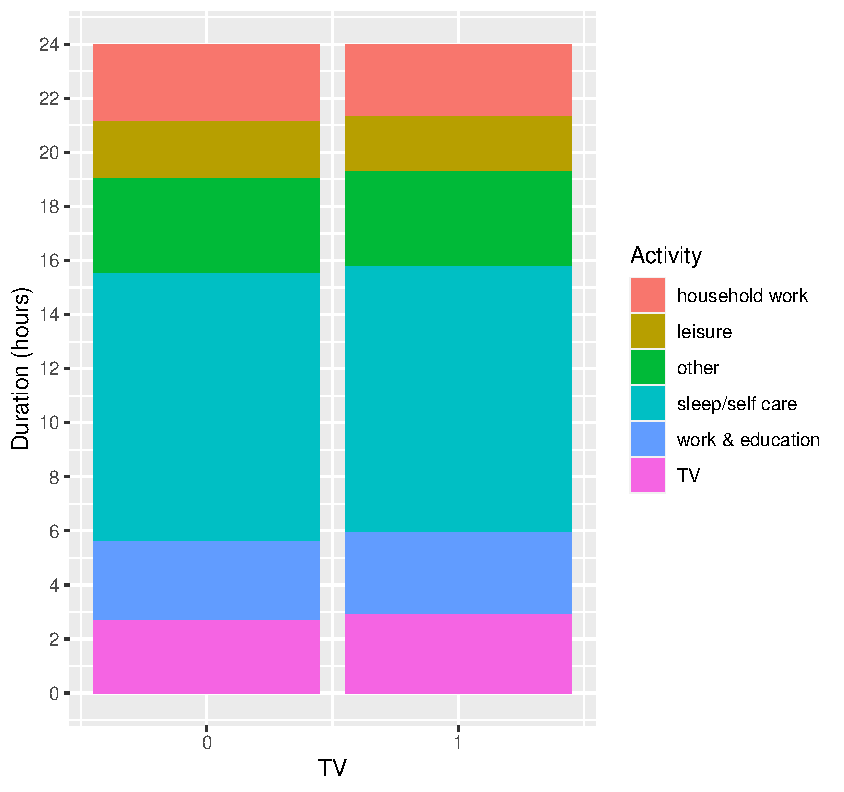
\includegraphics[width=.75\textwidth]{../../analysis/Output/graphs/time_breakdown.pdf}\\
\end{center}
\vspace{-5pt}
\footnotesize Hispanics with and without SLTV \hyperlink{atus_time}{\beamergotobutton{Back}}

\end{frame}




\begin{frame}
\frametitle{Differential effect of SLTV by program content} \label{transcript_calc}
\begin{center}
\scalebox{.8}{
	\begin{threeparttable}
			\begin{tabular}{lcccccccccc}
				\hline\hline\addlinespace
%				& \multicolumn{4}{c}{\textit{Minutes of TV watched}}  \\  				\cmidrule(lr){2-5} 
				&  (1) & (2) & (3)  \\
				\addlinespace\hline\addlinespace
				\multicolumn{3}{l}{Panel B: IHS(calculus taken)} \\ %edu_dda_appOLSIHS_spec3
                              	\hline\addlinespace
				 TV $\times$ Hispanic $\times$ \% programs on identity & 2.788$^{***}$ &  &  \\ 
				  & (1.034) &  &  \\ 
				 TV $\times$ Hispanic $\times$ \% programs on education &  & 0.829 &  \\ 
				  &  & (0.666) &  \\ 
				 TV $\times$ Hispanic $\times$ \% programs with role models &  &  & 1.616 \\ 
				  &  &  & (2.463) \\ 
				\hline\hline\addlinespace
				\# Hispanic, Asian students & Yes & Yes  & Yes\\
                                	School size controls & No & Yes & Yes\\
                                	School type controls & No & No & Yes \\
					\addlinespace\hline\hline
			\end{tabular}
			\begin{tablenotes}[flushleft]
				\item \textit{Notes:}  School district fixed effects are always included. Standard errors are clustered at the school district level. \hyperlink{transcript_sat}{\beamergotobutton{Back}}
			\end{tablenotes}
		\end{threeparttable}
        }
\end{center}
\end{frame}

\begin{frame}
\frametitle{Differential effect of SLTV by program content} \label{transcript_ap}
\begin{center}
\scalebox{.8}{
	\begin{threeparttable}
			\begin{tabular}{lcccccccccc}
				\hline\hline\addlinespace
%				& \multicolumn{4}{c}{\textit{Minutes of TV watched}}  \\  				\cmidrule(lr){2-5} 
				&  (1) & (2) & (3)  \\
				\addlinespace\hline\addlinespace
				\multicolumn{3}{l}{Panel C: IHS(APs passed)} \\ %edu_dda_calcOLSIHS_spec3
                              	\hline\addlinespace
				 TV $\times$ Hispanic $\times$ \% programs on identity & 1.721 &  &  \\ 
				  & (1.280) &  &  \\
				 TV $\times$ Hispanic $\times$ \% programs on education &  & 0.903 &  \\ 
				  &  & (0.922) &  \\ 
				 TV $\times$ Hispanic $\times$ \% programs with role models &  &  & $-$1.184 \\ 
				  &  &  & (2.989) \\ 
				\hline\hline\addlinespace
				\# Hispanic, Asian students & Yes & Yes  & Yes\\
                                	School size controls & No & Yes & Yes\\
                                	School type controls & No & No & Yes \\
					\addlinespace\hline\hline
			\end{tabular}
			\begin{tablenotes}[flushleft]
				\item \textit{Notes:}  School district fixed effects are always included. Standard errors are clustered at the school district level. \hyperlink{transcript_sat}{\beamergotobutton{Back}}
			\end{tablenotes}
		\end{threeparttable}
        }
\end{center}
\end{frame}

\begin{frame}
\frametitle{Effect of SLTV on foot traffic} \label{mech_placebo}
\begin{center}
\scalebox{.8}{
	\begin{threeparttable}
			\begin{tabular}{lcccccccccc}
				\hline\hline\addlinespace
%				& \multicolumn{4}{c}{\textit{Minutes of TV watched}}  \\  				\cmidrule(lr){2-5} 
				&  (1) & (2) & (3)  \\
				\addlinespace\hline\addlinespace
				\multicolumn{3}{l}{Panel A: IHS(IDEA (disability) students)} \\ %edu_dda_satactOLSIHS_spec3
                              	\hline\addlinespace
				TV dummy $\times$ Hispanic & 0.0318 & 0.0325 & 0.0318\\
  &(0.0338) & (0.0339) & (0.0338)\\
				\hline\hline\addlinespace
				\multicolumn{3}{l}{Panel B: IHS(bullied based on sex)} \\ %edu_dda_calcOLSIHS_spec3
                              	\hline\addlinespace
				TV dummy $\times$ Hispanic & 0.0090 & 0.0088 & 0.0088\\
  &(0.0056) & (0.0055) & (0.0055)\\	 
				\hline\hline\addlinespace
				\# Hispanic, Asian students & Yes & Yes  & Yes\\
                                	School size controls & No & Yes & Yes\\
                                	School type controls & No & No & Yes \\
					\addlinespace\hline\hline
			\end{tabular}
			\begin{tablenotes}[flushleft]
				\item \textit{Notes:}  School district fixed effects are always included. Standard errors are clustered at the school district level. \hyperlink{mech_main}{\beamergotobutton{Back}}
			\end{tablenotes}
		\end{threeparttable}
        }
\end{center}
\end{frame}

\begin{frame}
\frametitle{Effect of SLTV on foot traffic to Brazilian establishments} \label{safegraph_brazil}
\begin{center}
\scalebox{.8}{
	\begin{threeparttable}
			\begin{tabular}{lcccccccccc}
				\hline\hline\addlinespace
				& \multicolumn{4}{c}{\textit{IHS(visitors to location)}}  \\  				
				\cmidrule(lr){2-5} &  (1) & (2) & (3) & (4) \\
				\addlinespace\hline\addlinespace
				\multicolumn{4}{l}{Panel A.2: Restaurants --- Brazilian establishment indicator} \\ 
                              	\hline\addlinespace
				Hispanic $\times$ TV $\times$ Brazilian food&   0.058   &       0.058   &       0.058   &       0.058   \\
                    &     (0.241)   &     (0.241)   &     (0.241)   &     (0.241)   \\
				\hline\hline\addlinespace
				\multicolumn{4}{l}{Panel B.2: Recreation --- Brazilian establishment indicator} \\
                              	\hline\addlinespace
					Hispanic $\times$ TV $\times$ Brazilian brand&      0.328 & 0.328 & 0.328 & 0.328 \\
		                    &     (0.598)   &     (0.598)   &     (0.599)   &     (0.610)   \\
				\hline\hline\addlinespace
				County log(income) & Yes & Yes & Yes & Yes \\
				County \% Hispanic & No & Yes & Yes & Yes \\
				County log(pop.) & No & No & Yes & Yes \\
				County FE & No & No & No & Yes \\
				NAICS code FE & No & No & No & Yes \\
					\addlinespace\hline\hline
			\end{tabular}
			\begin{tablenotes}[flushleft]
				\item \textit{Notes:}  Standard errors are clustered at the county level. \hyperlink{safegraph_main}{\beamergotobutton{Back}}
			\end{tablenotes}
		\end{threeparttable}
        }
\end{center}
\end{frame}


\begin{frame}
\frametitle{Effect of SLTV on foot traffic to Japanese establishments} \label{safegraph_japan}
\begin{center}
\scalebox{.8}{
	\begin{threeparttable}
			\begin{tabular}{lcccccccccc}
				\hline\hline\addlinespace
				& \multicolumn{4}{c}{\textit{IHS(visitors to location)}}  \\  				
				\cmidrule(lr){2-5} &  (1) & (2) & (3) & (4) \\
				\addlinespace\hline\addlinespace
				\multicolumn{4}{l}{Panel A.3: Restaurants --- Japanese establishment indicator} \\ 
                              	\hline\addlinespace
				TV $\times$ Hispanic $\times$ Japanese food&        0.010   &       0.010   &       0.010   &       0.010   \\
                    &     (0.067)   &     (0.067)   &     (0.067)   &     (0.067)   \\
				\hline\hline\addlinespace
				\multicolumn{4}{l}{Panel B.3: Recreation --- Japanese establishment indicator} \\
                              	\hline\addlinespace
				TV $\times$ Hispanic $\times$ Japanese brand&        0.702   &       0.702   &       0.702   &       0.702   \\
                    &     (0.528)   &     (0.528)   &     (0.528)   &     (0.528)   \\
				\hline\hline\addlinespace
				County log(income) & Yes & Yes & Yes & Yes \\
				County \% Hispanic & No & Yes & Yes & Yes \\
				County log(pop.) & No & No & Yes & Yes \\
				County FE & No & No & No & Yes \\
				NAICS code FE & No & No & No & Yes \\
					\addlinespace\hline\hline
			\end{tabular}
			\begin{tablenotes}[flushleft]
				\item \textit{Notes:}  Standard errors are clustered at the county level. \hyperlink{safegraph_main}{\beamergotobutton{Back}} 
			\end{tablenotes}
		\end{threeparttable}
        }
\end{center}
\end{frame}


\begin{frame}
\frametitle{Effect of SLTV on foot traffic to Cajun/Creole establishments} \label{safegraph_creole}
\begin{center}
\scalebox{.8}{
	\begin{threeparttable}
			\begin{tabular}{lcccccccccc}
				\hline\hline\addlinespace
				& \multicolumn{4}{c}{\textit{IHS(visitors to location)}}  \\  				
				\cmidrule(lr){2-5} &  (1) & (2) & (3) & (4) \\
				\addlinespace\hline\addlinespace
				\multicolumn{4}{l}{Panel A.4: Restaurants --- Cajun and Creole establishment indicator} \\ 
                              	\hline\addlinespace
				TV $\times$ Hispanic $\times$ Cajun and Creole food&       0.174   &       0.174   &       0.174   &       0.174   \\
                    &     (0.196)   &     (0.196)   &     (0.196)   &     (0.196)   \\
				\hline\hline\addlinespace
				\multicolumn{4}{l}{Panel B.4: Recreation --- Cajun and Creole establishment indicator} \\ 
                              	\hline\addlinespace
				TV $\times$ Hispanic $\times$ Cajun and Creole brand&      -0.187 & -0.187 & -0.187 & -0.187 \\
				& (1.630)  & (1.630)& (1.630) & (1.631) \\
				\hline\hline\addlinespace
				County log(income) & Yes & Yes & Yes & Yes \\
				County \% Hispanic & No & Yes & Yes & Yes \\
				County log(pop.) & No & No & Yes & Yes \\
				County FE & No & No & No & Yes \\
				NAICS code FE & No & No & No & Yes \\
					\addlinespace\hline\hline
			\end{tabular}
			\begin{tablenotes}[flushleft]
				\item \textit{Notes:}  Standard errors are clustered at the county level. \hyperlink{safegraph_main}{\beamergotobutton{Back}} 
			\end{tablenotes}
		\end{threeparttable}
        }
\end{center}
\end{frame}



\end{document}


























